\FILENAME

\section{Apache Hadoop using Docker}


In this section we will explore the 
Map/Reduce framework using Hadoop provided through a Docker
container. The example that we use in this session is similar to
WordCount but simple calculations are added e.g. minimum, maximum,
average and standard deviation values using several input files which
contain float numbers.

\subsection{Draft: Creating the Hadoop Container}

\TODO{Hyungro: Please provide the Dockerfile and explain how to create
  the Docker image locally. Than use that image to do the next
  examples.}


\subsection{Hadoop from Docker}

We use a Docker image from Docker Hub:
(\url{https://hub.docker.com/r/lee212/e222/}) The base image is from
sequenceiq/hadoop and the example with input data is added for this
tutorial.

\subsection{Start a Hadoop container}

\begin{lstlisting}
docker run -it lee212/e222 /etc/bootstrap.sh -bash
\end{lstlisting}

It may take a few minutes at first to download image layers which are
about 847MB.

\subsection{Statistical Example with Hadoop}       

After a container is launched, the interactive shell prompt is given
to run hadoop application which we have an example to get
Min/Max/Avg/Std values by analyzing input text files.

\subsubsection{Description}

In a nutshell, this Hadoop program reads multiple files from HDFS and
provides calculated values. We walk through every step from compiling
Java source code to reading a output file from HDFS. The idea of this
exercise is to get you started with Hadoop and the MapReduce
concept. You may seen the WordCount from Hadoop official website or
documentation and this example has a same functions (Map/Reduce)
except that you will be computing the basic statistics such as min,
max, average, and standard deviation of a given data set.

The input to the program will be a text file(s) carrying exactly one
floating point number per line. The result file includes \textit{min,
  max, average, and standard deviation} of these numbers.


  \begin{figure}[!htbp]
    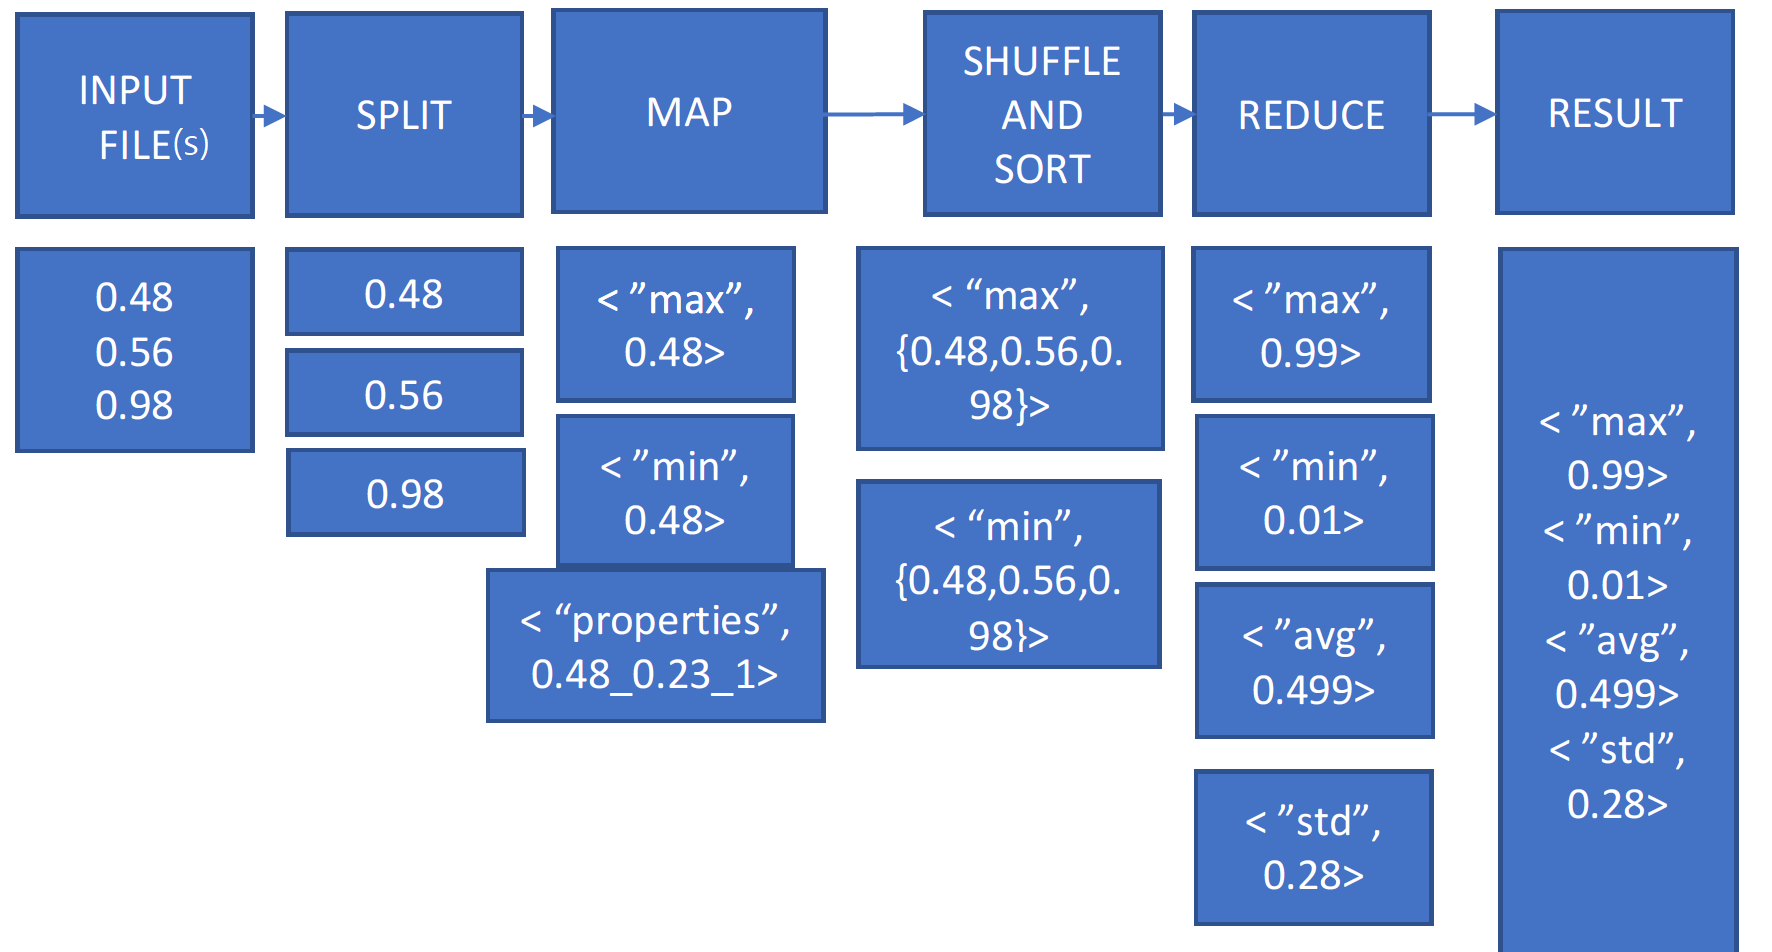
\includegraphics[width=8cm,height=8cm]{section/container/images/docker-hadoop-1.png}
    \centering
  \end{figure}

\subsubsection{Base Location}

The example is available at:

\begin{lstlisting}
cd /cloudmesh/exer1
\end{lstlisting}

\subsubsection{Input Files}

A test input files are available under
\verb|/cloudmesh/exer1/input_data}|
directory inside of the container.  The statistics values for this
input are \textit{Min: 0.20 Max: 19.99 Avg: 9.51 StdDev: 5.55} for all
input files.

10 files contain 55000 lines to process and each line is a random
float point value ranging from 0.2 to 20.0.

\subsubsection{Compilation}

The source code file name is \textit{MinMaxAvgStd.java} which is
available at \textit{/cloudmesh/exer1/src/exercise/}.

There are three functions in the code \textit{Map, Reduce and Main}
where Map reads each line of a file and updates values to calculate
minimum, maximum values and Reduce collects mappers to produce average
and standard deviation values at last.

\begin{lstlisting}
export HADOOP_CLASSPATH=`$HADOOP_PREFIX/bin/hadoop classpath`
mkdir /cloudmesh/exer1/dest
javac -classpath $HADOOP_CLASSPATH -d /cloudmesh/exer1/dest /cloudmesh/exer1/src/exercise/MinMaxAvgStd.java
\end{lstlisting}

These commands simply prepare compiling the example code and the
compiled class files are generated at the \textit{dest} location.

\subsubsection{Archiving Class Files}

Jar command tool helps archiving classes in a single file which will be used
when Hadoop runs this example. This is useful because a jar file contains all
necessary files to run a program.

\begin{lstlisting}
jar -cvf exer1.jar -C /cloudmesh/exer1/dest/ /cloudmesh/exer1/
\end{lstlisting}

\subsubsection{HDFS for Input/Output}

The input files need to be uploaded to HDFS as Hadoop runs this example by
reading input files from HDFS.

\begin{lstlisting}
export PATH=$PATH:/$HADOOP_PREFIX/bin
hadoop fs -mkdir exer1_input
hadoop fs -put input_data/* exer1_input
hadoop fs -ls exer1_input/
\end{lstlisting}

If uploading is completed, you may see file listings like:

\begin{lstlisting}
Found 10 items
-rw-r--r--   1 root supergroup      13942 2018-02-28 23:16 exer1_input/data_1000.txt
-rw-r--r--   1 root supergroup     139225 2018-02-28 23:16 exer1_input/data_10000.txt
-rw-r--r--   1 root supergroup      27868 2018-02-28 23:16 exer1_input/data_2000.txt
-rw-r--r--   1 root supergroup      41793 2018-02-28 23:16 exer1_input/data_3000.txt
-rw-r--r--   1 root supergroup      55699 2018-02-28 23:16 exer1_input/data_4000.txt
-rw-r--r--   1 root supergroup      69663 2018-02-28 23:16 exer1_input/data_5000.txt
-rw-r--r--   1 root supergroup      83614 2018-02-28 23:16 exer1_input/data_6000.txt
-rw-r--r--   1 root supergroup      97490 2018-02-28 23:16 exer1_input/data_7000.txt
-rw-r--r--   1 root supergroup     111451 2018-02-28 23:16 exer1_input/data_8000.txt
-rw-r--r--   1 root supergroup     125337 2018-02-28 23:16 exer1_input/data_9000.txt
\end{lstlisting}

\subsubsection{Run Program with a Single Input File}

We are ready to run the program to calculate values from text
files. First, we simply run the program with a single input file to
see how it works.  \verb|data_1000.txt| contains 1000 lines of
floats, we use this file here.

\begin{lstlisting}
hadoop jar exer1.jar exercise.MinMaxAvgStd exer1_input/data_1000.txt exer1_output_1000
\end{lstlisting}

The command runs with input parameters which indicate a jar file (the
program, exer1.jar), exercise.MinMaxAvgStd (package name.class name),
input file path (\verb|exer1_input/data_1000.txt|) and output file path
(\verb|exer1_output_1000|).

The sample results that the program produces look like this:

\begin{lstlisting}
18/02/28 23:48:50 INFO client.RMProxy: Connecting to ResourceManager at /0.0.0.0:8032
18/02/28 23:48:50 INFO input.FileInputFormat: Total input paths to process : 1
18/02/28 23:48:50 INFO mapreduce.JobSubmitter: number of splits:1
18/02/28 23:48:50 INFO mapreduce.JobSubmitter: Submitting tokens for job: job_1519877569596_0002
18/02/28 23:48:51 INFO impl.YarnClientImpl: Submitted application application_1519877569596_0002
18/02/28 23:48:51 INFO mapreduce.Job: The url to track the job: http://f5e82d68ba4a:8088/proxy/application_1519877569596_0002/
18/02/28 23:48:51 INFO mapreduce.Job: Running job: job_1519877569596_0002
18/02/28 23:48:56 INFO mapreduce.Job: Job job_1519877569596_0002 running in uber mode : false
18/02/28 23:48:56 INFO mapreduce.Job:  map 0% reduce 0%
18/02/28 23:49:00 INFO mapreduce.Job:  map 100% reduce 0%
18/02/28 23:49:05 INFO mapreduce.Job:  map 100% reduce 100%
18/02/28 23:49:05 INFO mapreduce.Job: Job job_1519877569596_0002 completed successfully
18/02/28 23:49:05 INFO mapreduce.Job: Counters: 49
        File System Counters
                FILE: Number of bytes read=81789
                FILE: Number of bytes written=394101
                FILE: Number of read operations=0
                FILE: Number of large read operations=0
                FILE: Number of write operations=0
                HDFS: Number of bytes read=14067
                HDFS: Number of bytes written=86
                HDFS: Number of read operations=6
                HDFS: Number of large read operations=0
                HDFS: Number of write operations=2
        Job Counters
                Launched map tasks=1
                Launched reduce tasks=1
                Data-local map tasks=1
                Total time spent by all maps in occupied slots (ms)=2107
                Total time spent by all reduces in occupied slots (ms)=2316
                Total time spent by all map tasks (ms)=2107
                Total time spent by all reduce tasks (ms)=2316
                Total vcore-seconds taken by all map tasks=2107
                Total vcore-seconds taken by all reduce tasks=2316
                Total megabyte-seconds taken by all map tasks=2157568
                Total megabyte-seconds taken by all reduce tasks=2371584
        Map-Reduce Framework
                Map input records=1000
                Map output records=3000
                Map output bytes=75783
                Map output materialized bytes=81789
                Input split bytes=125
                Combine input records=0
                Combine output records=0
                Reduce input groups=3
                Reduce shuffle bytes=81789
                Reduce input records=3000
                Reduce output records=4
                Spilled Records=6000
                Shuffled Maps =1
                Failed Shuffles=0
                Merged Map outputs=1
                GC time elapsed (ms)=31
                CPU time spent (ms)=1440
                Physical memory (bytes) snapshot=434913280
                Virtual memory (bytes) snapshot=1497260032
                Total committed heap usage (bytes)=402653184
        Shuffle Errors
                BAD_ID=0
                CONNECTION=0
                IO_ERROR=0
                WRONG_LENGTH=0
                WRONG_MAP=0
                WRONG_REDUCE=0
        File Input Format Counters
                Bytes Read=13942
        File Output Format Counters
                Bytes Written=86

\end{lstlisting}

The second line of the following logs indicates that the number of
input files is 1.

\subsubsection{Result for Single Input File}

We reads results from HDFS by:

\begin{lstlisting}
doop fs -cat exer1_output_1000/part-r-00000
\end{lstlisting}

The sample output looks like:

\begin{lstlisting}
Max:    19.9678704297
Min:    0.218880718983
Avg:    10.225467263249385
Std:    5.679809322880863
\end{lstlisting}

\subsubsection{Run Program with Multiple Input Files}

The first run was done pretty quickly (1440 milliseconds took
according to the sample result above) because the input file size was
small (1,000 lines) and it was a single file. We provides more input
files with a larger size (2,000 to 10,000 lines). Input files are
already uploaded to HDFS. We simply run the program again with a
slight change in the parameters.

\begin{lstlisting}
hadoop jar exer1.jar exercise.MinMaxAvgStd exer1_input/ exer1_output_all
\end{lstlisting}

The command is almost same except that an input path is a directory
and a new output directory.  Note that every time that you run this
program, the output directory will be created which means that you
have to provide a new directory name unless you delete it.

The sample output messages look like the following which is almost
identical compared to the previous run except that this time the
number of input files to process is 10, see the line two below:

\begin{lstlisting}
18/02/28 23:17:18 INFO client.RMProxy: Connecting to ResourceManager at /0.0.0.0:8032
18/02/28 23:17:18 INFO input.FileInputFormat: Total input paths to process : 10
18/02/28 23:17:18 INFO mapreduce.JobSubmitter: number of splits:10
18/02/28 23:17:18 INFO mapreduce.JobSubmitter: Submitting tokens for job: job_1519877569596_0001
18/02/28 23:17:19 INFO impl.YarnClientImpl: Submitted application application_1519877569596_0001
18/02/28 23:17:19 INFO mapreduce.Job: The url to track the job: http://f5e82d68ba4a:8088/proxy/application_1519877569596_0001/
18/02/28 23:17:19 INFO mapreduce.Job: Running job: job_1519877569596_0001
18/02/28 23:17:24 INFO mapreduce.Job: Job job_1519877569596_0001 running in uber mode : false
18/02/28 23:17:24 INFO mapreduce.Job:  map 0% reduce 0%
18/02/28 23:17:32 INFO mapreduce.Job:  map 40% reduce 0%
18/02/28 23:17:33 INFO mapreduce.Job:  map 60% reduce 0%
18/02/28 23:17:36 INFO mapreduce.Job:  map 70% reduce 0%
18/02/28 23:17:37 INFO mapreduce.Job:  map 100% reduce 0%
18/02/28 23:17:39 INFO mapreduce.Job:  map 100% reduce 100%
18/02/28 23:17:39 INFO mapreduce.Job: Job job_1519877569596_0001 completed successfully
18/02/28 23:17:39 INFO mapreduce.Job: Counters: 49
        File System Counters
                FILE: Number of bytes read=4496318
                FILE: Number of bytes written=10260627
                FILE: Number of read operations=0
                FILE: Number of large read operations=0
                FILE: Number of write operations=0
                HDFS: Number of bytes read=767333
                HDFS: Number of bytes written=84
                HDFS: Number of read operations=33
                HDFS: Number of large read operations=0
                HDFS: Number of write operations=2
        Job Counters
                Launched map tasks=10
                Launched reduce tasks=1
                Data-local map tasks=10
                Total time spent by all maps in occupied slots (ms)=50866
                Total time spent by all reduces in occupied slots (ms)=4490
                Total time spent by all map tasks (ms)=50866
                Total time spent by all reduce tasks (ms)=4490
                Total vcore-seconds taken by all map tasks=50866
                Total vcore-seconds taken by all reduce tasks=4490
                Total megabyte-seconds taken by all map tasks=52086784
                Total megabyte-seconds taken by all reduce tasks=4597760
        Map-Reduce Framework
                Map input records=55000
                Map output records=165000
                Map output bytes=4166312
                Map output materialized bytes=4496372
                Input split bytes=1251
                Combine input records=0
                Combine output records=0
                Reduce input groups=3
                Reduce shuffle bytes=4496372
                Reduce input records=165000
                Reduce output records=4
                Spilled Records=330000
                Shuffled Maps =10
                Failed Shuffles=0
                Merged Map outputs=10
                GC time elapsed (ms)=555
                CPU time spent (ms)=16040
                Physical memory (bytes) snapshot=2837708800
                Virtual memory (bytes) snapshot=8200089600
                Total committed heap usage (bytes)=2213019648
        Shuffle Errors
                BAD_ID=0
                CONNECTION=0
                IO_ERROR=0
                WRONG_LENGTH=0
                WRONG_MAP=0
                WRONG_REDUCE=0
        File Input Format Counters
                Bytes Read=766082
        File Output Format Counters
                Bytes Written=84
\end{lstlisting}


\subsubsection{Result for Multiple Files}

\begin{lstlisting}
hadoop fs -cat exer1_output_all/part-r-00000
\end{lstlisting}

The expected result looks like:

\begin{lstlisting}
Max:    19.999191254
Min:    0.200268613863
Avg:    9.514884854468903
Std:    5.553921579413547
\end{lstlisting}

\subsection{Conclusion}

The example program of calculating some values by reading multiple
files shows how Map/Reduce is written by a Java programming language
and how Hadoop runs its program using HDFS. We also observed the one
of benefits using Docker container which is that the hassle of
configuration and installation of Hadoop is not necessary anymore.


